\documentclass{article}

% Packages required to support encoding
\usepackage{ucs}
\usepackage[utf8x]{inputenc}
\usepackage{graphicx} 
% Packages required by code

% Packages always used
\usepackage{listings}
\usepackage{hyperref}
\usepackage{xspace}
\usepackage[usenames,dvipsnames]{color}
\hypersetup{colorlinks=true,urlcolor=blue}


\usepackage[framed,numbered,autolinebreaks,useliterate] {mcode}


\usepackage{geometry}
\geometry{letterpaper,textwidth=350pt,textheight=680pt,tmargin=60pt,
            left=72pt,footskip=24pt,headsep=18pt,headheight=14pt}
\usepackage{amsmath}
\usepackage{amssymb}
\usepackage{textcase}
\usepackage{soul}

\newcommand{\mat}[1]{\boldsymbol{#1}}\renewcommand{\vec}[1]{\boldsymbol{\mathrm{#1}}}
\newcommand{\vecalt}[1]{\boldsymbol{#1}}

\newcommand{\conj}[1]{\overline{#1}}

\newcommand{\normof}[1]{\|#1\|}
\newcommand{\onormof}[2]{\|#1\|_{#2}}

\newcommand{\itr}[2]{#1^{(#2)}}
\newcommand{\itn}[1]{^{(#1)}}

\newcommand{\eps}{\varepsilon}
\newcommand{\kron}{\otimes}

\DeclareMathOperator{\diag}{diag}
\DeclareMathOperator{\trace}{trace}
\DeclareMathOperator{\tvec}{vec}

\newcommand{\prob}{\mathbb{P}}
\newcommand{\probof}[1]{\prob\left\{ #1 \right\}}

\newcommand{\pmat}[1]{\begin{pmatrix} #1 \end{pmatrix}}
\newcommand{\bmat}[1]{\begin{bmatrix} #1 \end{bmatrix}}
\newcommand{\spmat}[1]{\left(\begin{smallmatrix} #1 \end{smallmatrix}\right)}
\newcommand{\sbmat}[1]{\left[\begin{smallmatrix} #1 \end{smallmatrix}\right]}

\newcommand{\RR}{\mathbb{R}}
\newcommand{\CC}{\mathbb{C}}

\providecommand{\eye}{\mat{I}}
\providecommand{\mA}{\ensuremath{\mat{A}}}
\providecommand{\mB}{\ensuremath{\mat{B}}}
\providecommand{\mC}{\ensuremath{\mat{C}}}
\providecommand{\mD}{\ensuremath{\mat{D}}}
\providecommand{\mE}{\ensuremath{\mat{E}}}
\providecommand{\mF}{\ensuremath{\mat{F}}}
\providecommand{\mG}{\ensuremath{\mat{G}}}
\providecommand{\mH}{\ensuremath{\mat{H}}}
\providecommand{\mI}{\ensuremath{\mat{I}}}
\providecommand{\mJ}{\ensuremath{\mat{J}}}
\providecommand{\mK}{\ensuremath{\mat{K}}}
\providecommand{\mL}{\ensuremath{\mat{L}}}
\providecommand{\mM}{\ensuremath{\mat{M}}}
\providecommand{\mN}{\ensuremath{\mat{N}}}
\providecommand{\mO}{\ensuremath{\mat{O}}}
\providecommand{\mP}{\ensuremath{\mat{P}}}
\providecommand{\mQ}{\ensuremath{\mat{Q}}}
\providecommand{\mR}{\ensuremath{\mat{R}}}
\providecommand{\mS}{\ensuremath{\mat{S}}}
\providecommand{\mT}{\ensuremath{\mat{T}}}
\providecommand{\mU}{\ensuremath{\mat{U}}}
\providecommand{\mV}{\ensuremath{\mat{V}}}
\providecommand{\mW}{\ensuremath{\mat{W}}}
\providecommand{\mX}{\ensuremath{\mat{X}}}
\providecommand{\mY}{\ensuremath{\mat{Y}}}
\providecommand{\mZ}{\ensuremath{\mat{Z}}}
\providecommand{\mLambda}{\ensuremath{\mat{\Lambda}}}
\providecommand{\mPbar}{\bar{\mP}}

\providecommand{\ones}{\vec{e}}
\providecommand{\va}{\ensuremath{\vec{a}}}
\providecommand{\vb}{\ensuremath{\vec{b}}}
\providecommand{\vc}{\ensuremath{\vec{c}}}
\providecommand{\vd}{\ensuremath{\vec{d}}}
\providecommand{\ve}{\ensuremath{\vec{e}}}
\providecommand{\vf}{\ensuremath{\vec{f}}}
\providecommand{\vg}{\ensuremath{\vec{g}}}
\providecommand{\vh}{\ensuremath{\vec{h}}}
\providecommand{\vi}{\ensuremath{\vec{i}}}
\providecommand{\vj}{\ensuremath{\vec{j}}}
\providecommand{\vk}{\ensuremath{\vec{k}}}
\providecommand{\vl}{\ensuremath{\vec{l}}}
\providecommand{\vm}{\ensuremath{\vec{l}}}
\providecommand{\vn}{\ensuremath{\vec{n}}}
\providecommand{\vo}{\ensuremath{\vec{o}}}
\providecommand{\vp}{\ensuremath{\vec{p}}}
\providecommand{\vq}{\ensuremath{\vec{q}}}
\providecommand{\vr}{\ensuremath{\vec{r}}}
\providecommand{\vs}{\ensuremath{\vec{s}}}
\providecommand{\vt}{\ensuremath{\vec{t}}}
\providecommand{\vu}{\ensuremath{\vec{u}}}
\providecommand{\vv}{\ensuremath{\vec{v}}}
\providecommand{\vw}{\ensuremath{\vec{w}}}
\providecommand{\vx}{\ensuremath{\vec{x}}}
\providecommand{\vy}{\ensuremath{\vec{y}}}
\providecommand{\vz}{\ensuremath{\vec{z}}}
\providecommand{\vpi}{\ensuremath{\vecalt{\pi}}}

\sodef\allcapsspacing{\upshape}{0.15em}{0.65em}{0.6em}%

\makeatletter
\def\maketitle{%
\par
\hrule height 0.75pt\vspace{1ex}
\par\noindent
\begin{minipage}{0.5\textwidth}
\scshape
purdue university $\cdot$ CS 580 \\
Introduction to the Analysis of Algorithms
\end{minipage}
\begin{minipage}{0.5\textwidth}
\raggedleft
\MakeTextUppercase{\allcapsspacing{\@title}}\\[0.2ex]
\textit{\@author}\\[0.2ex]
\textit{\@date}
\end{minipage}
\par\vspace{1ex}
\hrule height 1pt
\vspace{2ex}
\par
}
\makeatother

\author{Jun Cheng}
\title{Lecture Notes}
% auto generate a title
\AtBeginDocument{\maketitle}


\title{Homework}



\begin{document} 



\hypertarget{problem_0_homework_checklist_2}{}
\subsection*{{Problem 0: Homework checklist}}
\label{problem_0_homework_checklist_2}

\checkmark	I didn't talk with any one about this homework. \newline
\checkmark 	Source-code are included at the end of this document. 

\hypertarget{problem_0_homework_checklist_2}{}
\subsection*{{Problem 1}}
\label{problem_0_homework_checklist_2}

\begin{enumerate}
\item $\bmat{0 & 5 \\ 0 & 0}  = \bmat{1 & 0 \\ 0 & 1} \bmat{5 & 0 \\ 0 & 0 } \bmat{ 0 & 1 \\ -1 & 0 }$


\item $\bmat{5 & 0 \\ 2 & 0} = \bmat{0.92 & -0.37\\ 0.37& 0.92}\bmat{5.4& 0\\ 0& 0} \bmat{1 & 0 \\0 & 1} $


\item $\bmat{5 & -5 \\ 2 & -2 \\ 0 & 0}= \bmat{0.93 & -0.37 & 0 \\ 0.37 & 0.93 & 0 \\ 0 & 0 & 0 }\bmat{7.6 & 0 \\ 0 & 0 \\ 0 & 0 }
\bmat{0.707 & -0.707 \\ 0.707 & 0.707 } $


\item $\bmat{2 & 0 \\ 0 & -1} = \bmat{1 & 0 \\ 0 & 1} \bmat{2 & 0 \\ 0 & -1 } \bmat{1 & 0 \\ 0 & 1 }$

\end{enumerate}



\hypertarget{problem_0_homework_checklist_2}{}
\subsection*{{Problem 2: }}
\label{problem_0_homework_checklist_2}

\begin{enumerate}

\item 
For example, The matrix \\
\begin{align} 
\mA = \bmat{5 &-5 \\ 2 & -2} 
\end{align}
From Matlab SVD we can get: 
\begin{align} 
\mA =\bmat{5 & -5 \\ 2 & -2}= \bmat{-0.93 & -0.37  \\ -0.37 & 0.93   }\bmat{7.6 & 0 \\ 0 & 0 }
\bmat{-0.707 & -0.707 \\ 0.707 & -0.707 } 
\end{align}
But I got:
\begin{align} 
\mA = \bmat{5 & -5 \\ 2 & -2}= \bmat{0.93 & -0.37  \\ 0.37 & 0.93   }\bmat{7.6 & 0 \\ 0 & 0  }
\bmat{0.707 & -0.707 \\ 0.707 & 0.707 } 
\end{align}
That means matrix A has two different  decomposition, but in both cases they have the same singular value. \\
\item 

\item 
Suppose $\mA$ is a matrix with eigenvalues $\{\sigma_i\}$\\
The SVD of $\mA$ is $\mA=\mU \Sigma\mV^T $ where $\mU$ and $\mV$ are both orthogonal matrix. 

\begin{flalign} 
\mA^{-1} &= (\mU \Sigma\mV^T)^{-1}\\
&=(\mV^T)^{-1}\Sigma^{-1}\mU^{-1}\\
&=(\mV^T)^T\Sigma^{-1}\mU^T\\
&=\mV\Sigma^{-1}\mU^T &&
\end{flalign}
Then  $\mA^{-1}$ is a matrix with eigenvalues $\{\frac{1}{\sigma_i}\}$
\begin{flalign} 
\|\mA^{-1}\| &= max\{\frac{1}{\sigma_i}\} \\
& = \frac{1}{\sigma_{min}} \\
\end{flalign}

\item 
The SVD of $\mQ$ is $\mQ=\mU \Sigma\mV^T=\mQ \mI\mI^T $ where $\mI$ is an identity matrix and it is also an orthogonal matrix. \\
In particular, the singular value are all $1$. 

\end{enumerate}

\hypertarget{}{}
\subsection*{{Problem 3: }}
\label{}

\begin{enumerate} 
\item 
If $m<n$, we can use $\mA^{T}= (\mU\Sigma\mV^T)^{T} = \mV\Sigma\mU^T$ is still SVD. 

\item 
$\mA = diag(\sigma_1, \sigma_2, ...\sigma_n, 0, ...) $\\
Then the best diagonal rank $k$ approximation to $\mA$ is \\
 $\mA_k =diag(\sigma_1, \sigma_2, ...\sigma_k, 0, ...)$ \\
 We aussume $k<n$ since we want to do the lower rank approximation. \\
 Then  
 \begin{flalign}
 \|\mA-\mA_k\|_2  &= \|diag(\sigma_1, \sigma_2, ...\sigma_n, 0, ...) - diag(\sigma_1, \sigma_2, ...\sigma_k, 0, ...) \|_2\\
&= \| diag(0 , .., \sigma_{k+1}, ...\sigma_n, 0, ...) \|_2 \\
&= max\{\sigma_{k+1}, ...\sigma_n \}
\end{flalign}
The small least answer could be $\sigma_n$ which is the smallest singular value of $\mA$. \\
\item 

\begin{flalign} 
\|\mA-\mA_n\| &= \|\sum_{i=1}^{n}\sigma_i\vu_i\vv_i^T-\sum_{i=1}^{n}\sigma_i\vu_i\vv_i^T\|\\
& = 0\\
\end{flalign}



\item 
\begin{flalign} 
\|\mA-\mA_R\| &= \|\sum_{i=1}^{n}\sigma_i\vu_i\vv_i^T-\sum_{i=1}^{R}\sigma_i\vu_i\vv_i^T\|\\
& = \|\sum_{i=R+1}^{n}\sigma_i\vu_i\vv_i^T\|\\
& = max\{\sigma_i\}\\
\end{flalign}
When they have the same set of singular values, Then 
\begin{align} \|\mA-\mA_R\| = 0\\ 
\end{align}

\item 
\begin{flalign} 
\|\mA-\mA_k\| &= \|\sum_{i=1}^{n}\sigma_i\vu_i\vv_i^T-\sum_{i=1}^{k}\sigma_i\vu_i\vv_i^T\|\\
& = \|\sum_{i=k+1}^{n}\sigma_i\vu_i\vv_i^T\|\\
& = max\{\sigma_{k+1}, ..., \sigma_{n}\}\\
& = \sigma_{k+1}
\end{flalign}
$\sigma_{k+1}$ is the largest singular value of $\mA-\mA_k$ \\


\item 
Based on the definition of 2-norm, for any vectors: \\ 
\begin{flalign}
 \|\mA\|=\sup_{x\neq0}\frac{\|\mA x\|}{\|x\|}
 \end{flalign} 
We know 
\begin{align} 
\|(\mA-\mB)x\|<\sigma_{k+1} 
\end{align}
Then \begin{align}  \sigma_{k+1} > \sup_{x\neq0}\frac{\|(\mA-\mB) x\|}{\|x\|}\end{align} 
for any vector $x$. \\
Therefore \begin{align}  \|(\mA-\mB)x\|<\sigma_{k+1}\|x\| \end{align}  

\item 
For a vector $\vw$ in the null-space of \mB\ 
\begin{align}    \mB\vw=0 \end{align} 
Therefore \begin{align}  \|(\mA-\mB)\vw\|=  \|\mA\vw\| <\sigma_{k+1}\|\vw\|\end{align} 

\item 
For a vector $\vx \in span(\vv_1, ...., \vv_{k+1}) , $\\
\begin{flalign} \|\mA\| &=\sup_{x\neq0}\frac{\|\mA \vz\|}{\|\vz\|}\\
&= max\{\sigma_1, \sigma_2, ..., \sigma_k\} \\
&\leq\sigma_{k+1} \\
\end{flalign} 
Then \begin{align} \|\mA\vz\|\leq\sigma_{k+1}\|\vz\| \end{align} 


\item 
The dimension of the space where $\mA\vw $ is bounded above is $(n-k) $, and 
the dimension of the space where $\mA\vz $ is bounded above is $(k+1) $.  Because the sum of the dimensions of those two spaces is more than $n$, there must be a non-zero vector which belongs to two of the subspaces. And this is a contradiction.  \\

\item
Yes, I did. \\
\end{enumerate} 

\hypertarget{problem_0_homework_checklist_2}{}
\subsection*{{Problem 4: }}
\label{}
\begin{enumerate} 
\item 
The data is stored as a 3 dimension array $256\times 1100 \times 10$. \\
 For each digit, there are 1100 images.  Those images include 256 pixels with shape $16 by 16 $ \\ And the sample images are shown as below. \\
 \begin{figure}
 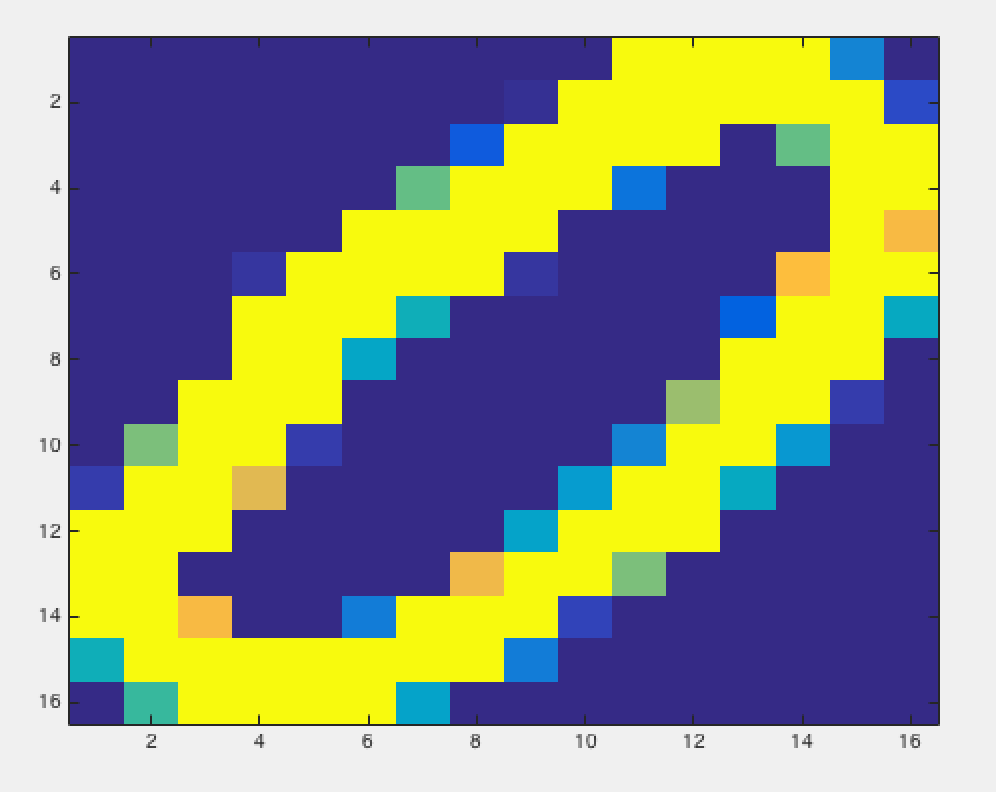
\includegraphics[width=0.25\textwidth, height=0.25\textwidth]{pic0}
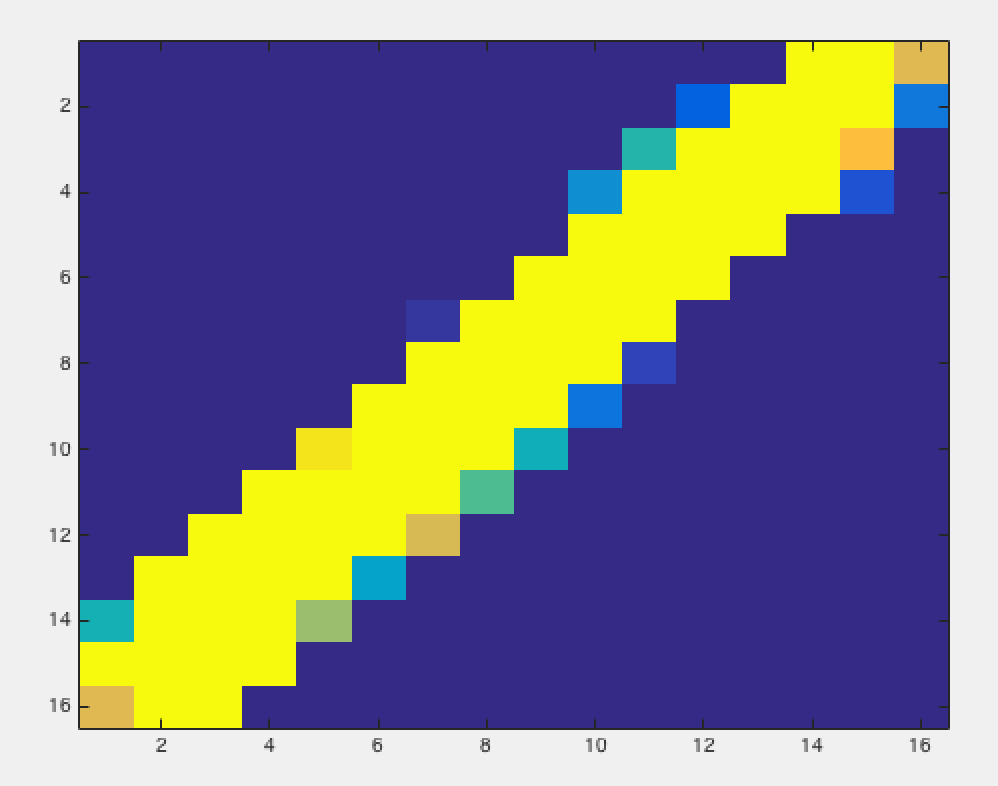
\includegraphics[width=0.25\textwidth, height=0.25\textwidth]{pic1}   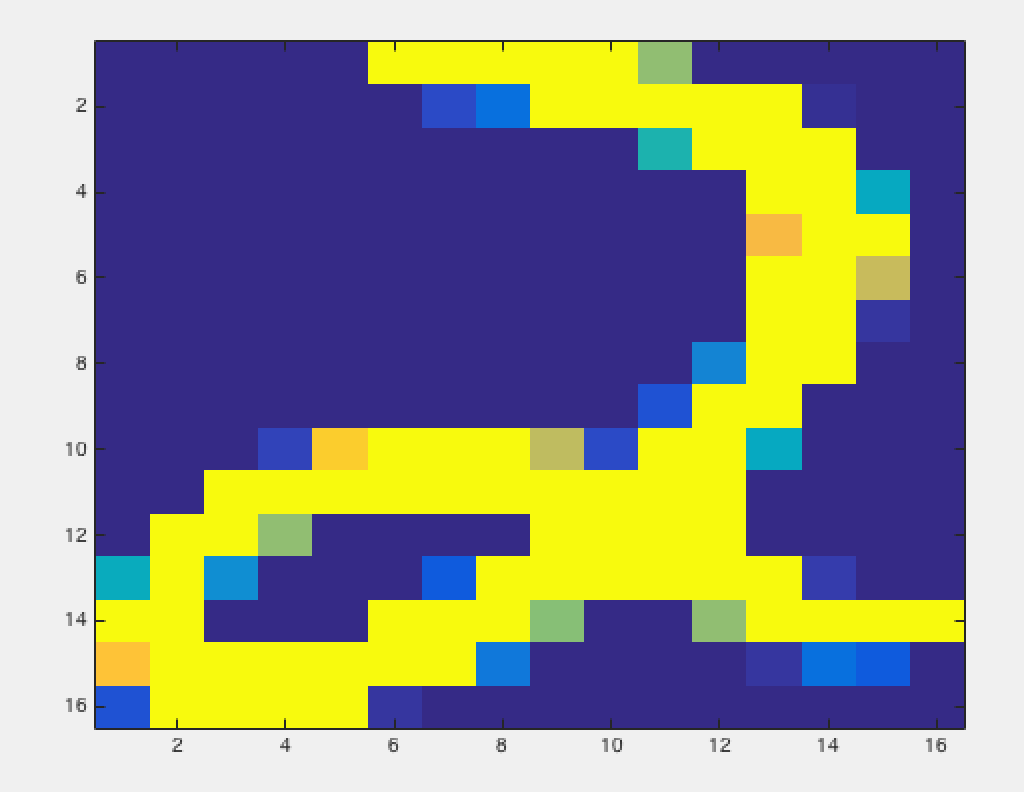
\includegraphics[width=0.25\textwidth, height=0.25\textwidth]{pic2}
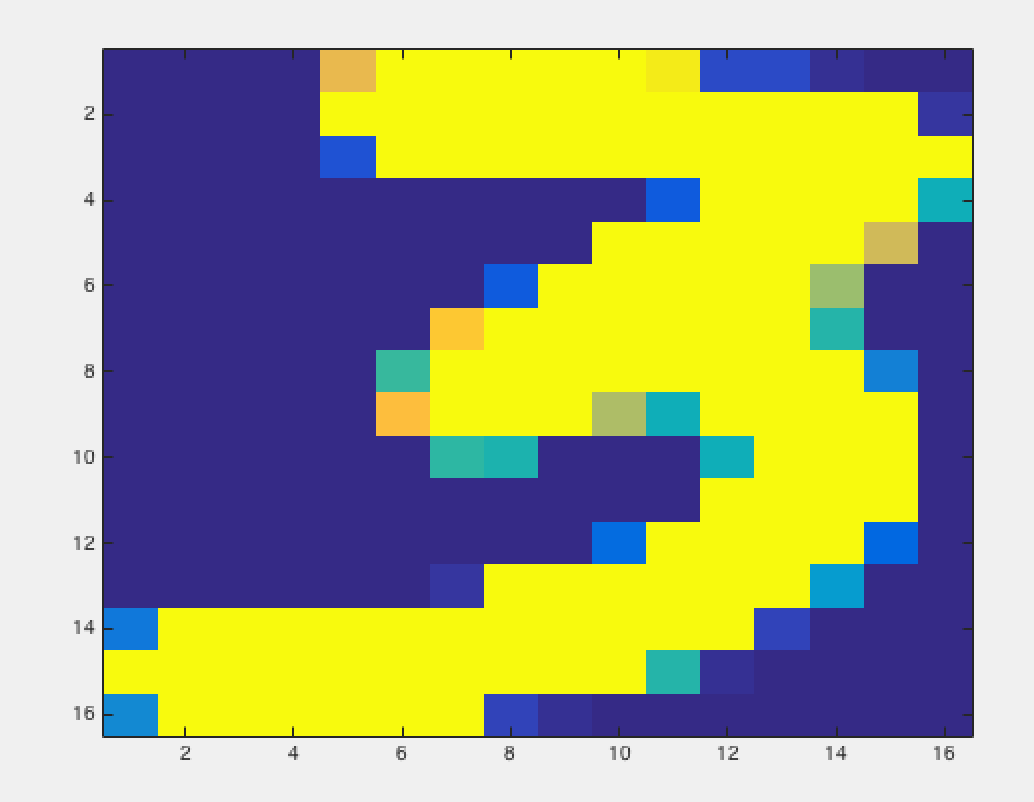
\includegraphics[width=0.25\textwidth, height=0.25\textwidth]{pic3}
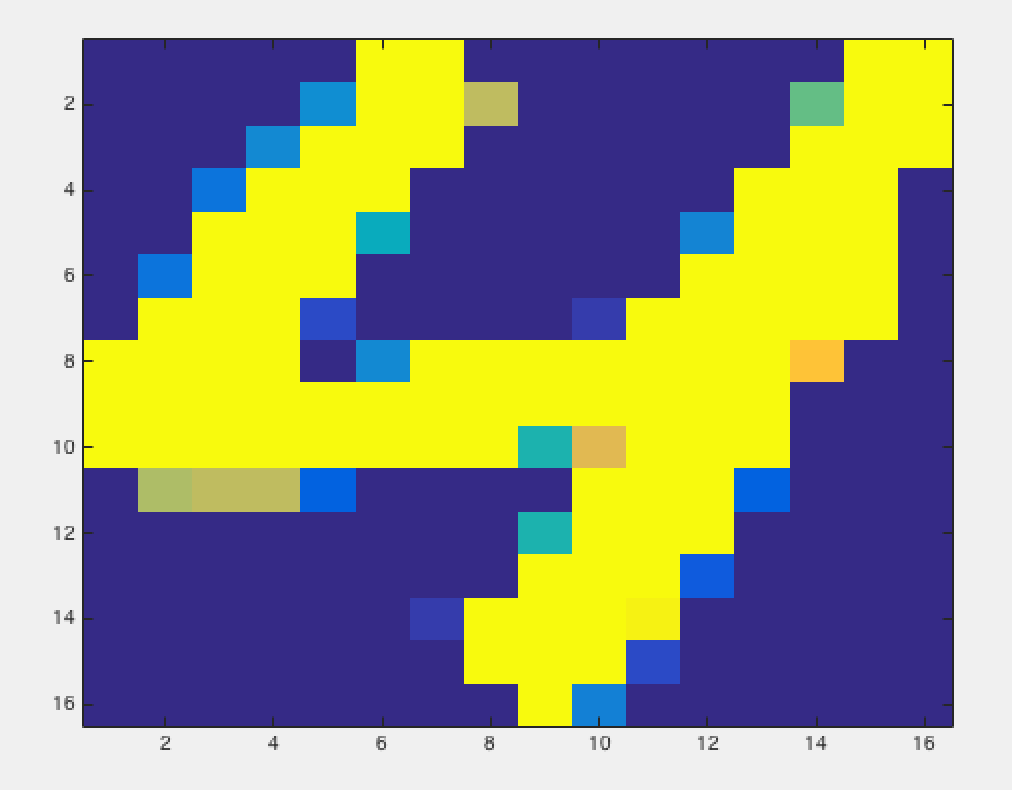
\includegraphics[width=0.25\textwidth, height=0.25\textwidth]{pic4}
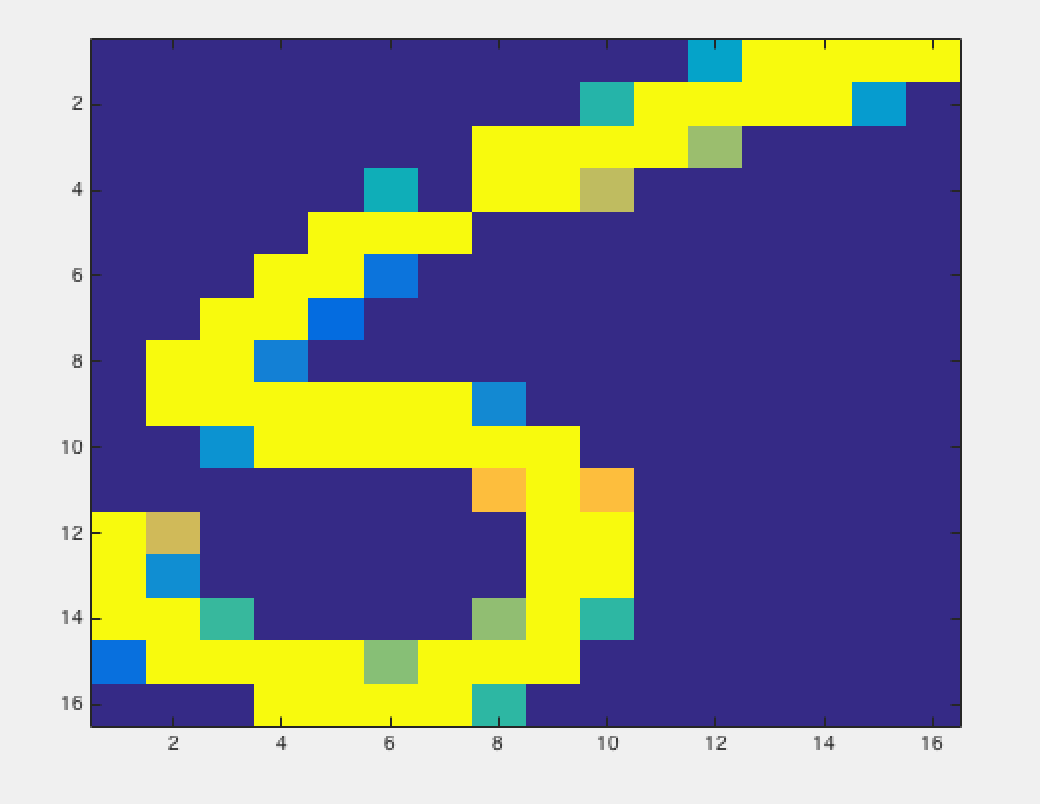
\includegraphics[width=0.25\textwidth, height=0.25\textwidth]{pic5}
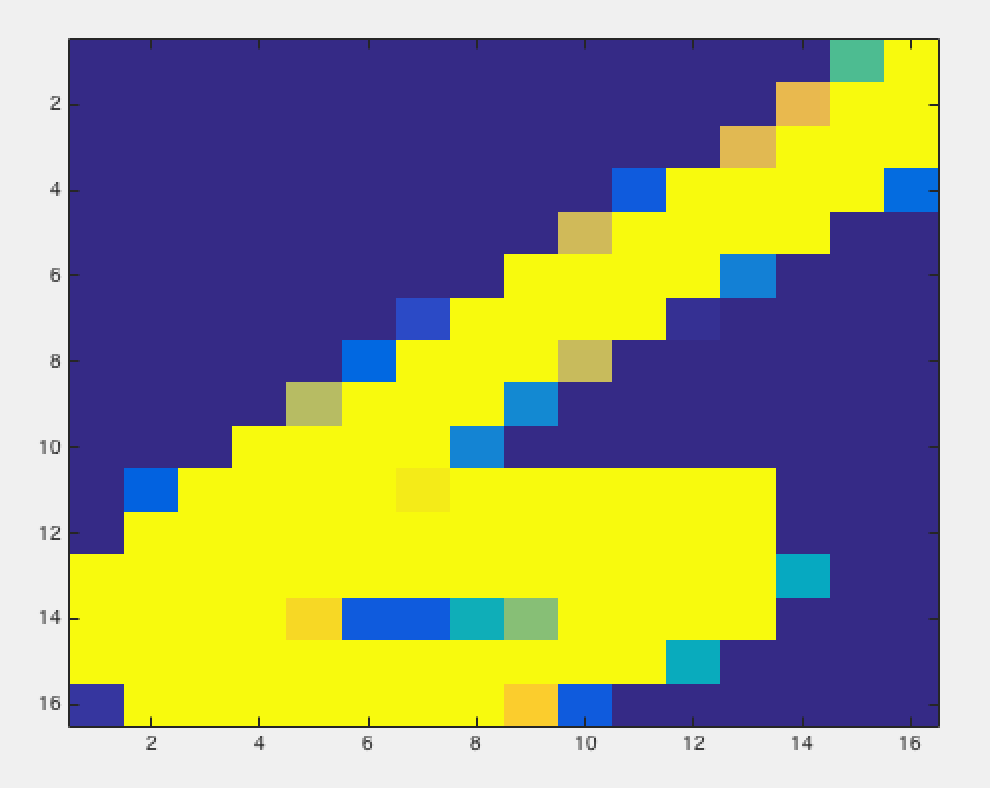
\includegraphics[width=0.25\textwidth, height=0.25\textwidth]{pic6}
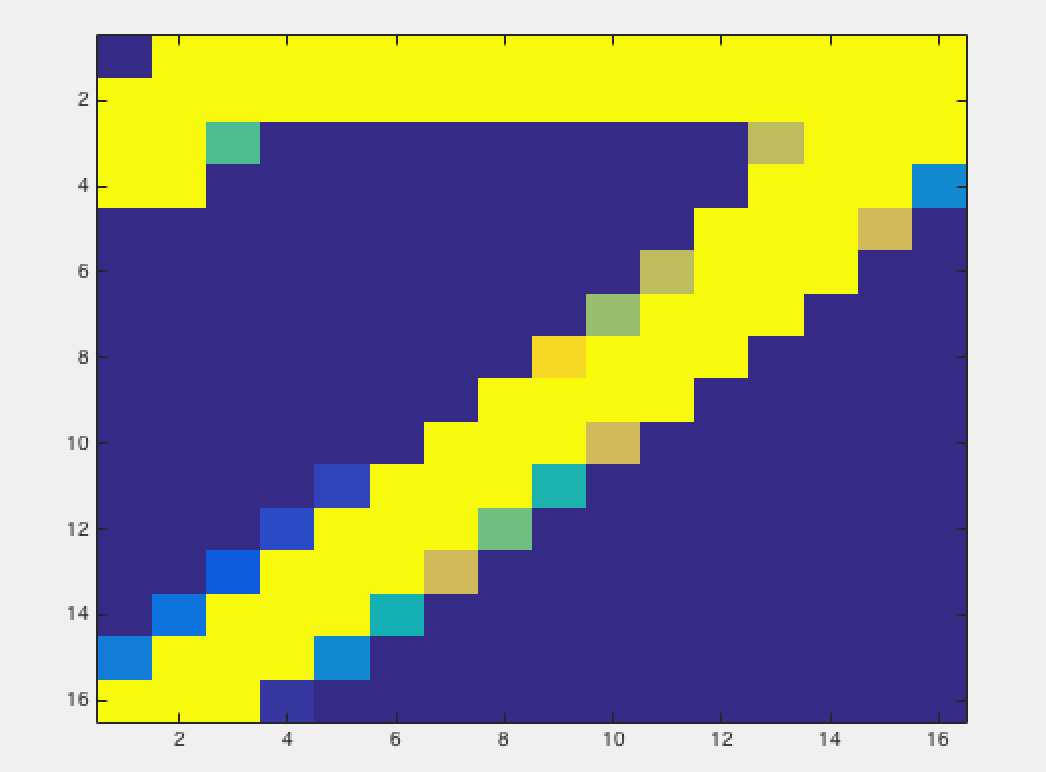
\includegraphics[width=0.25\textwidth, height=0.25\textwidth]{pic7}
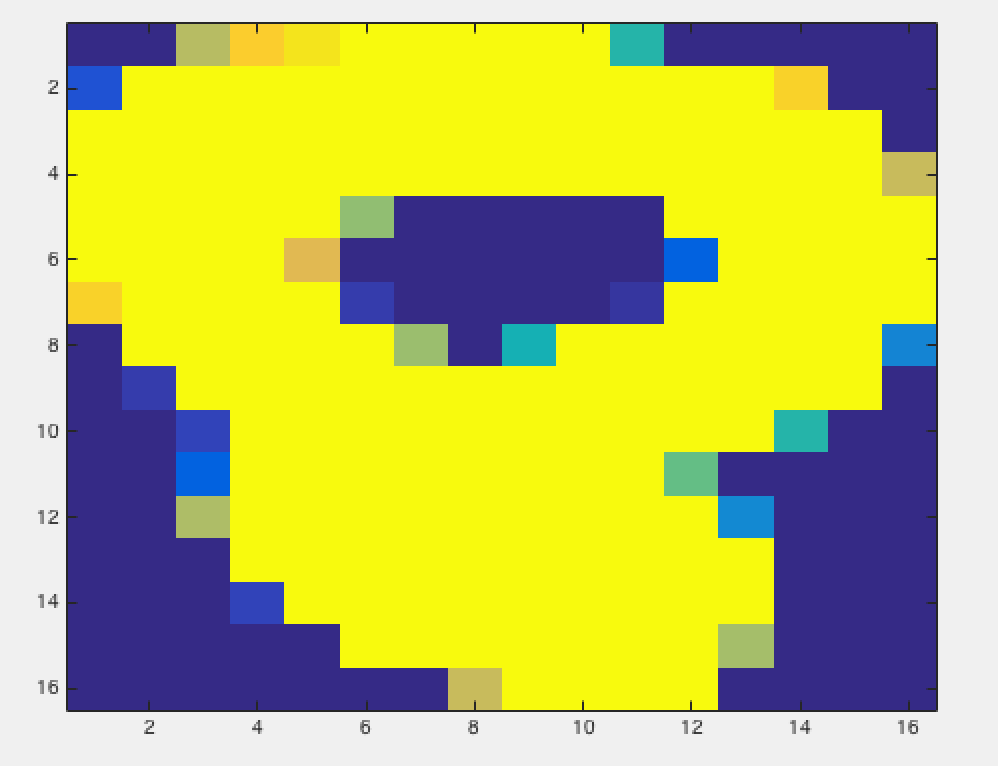
\includegraphics[width=0.25\textwidth, height=0.25\textwidth]{pic8}
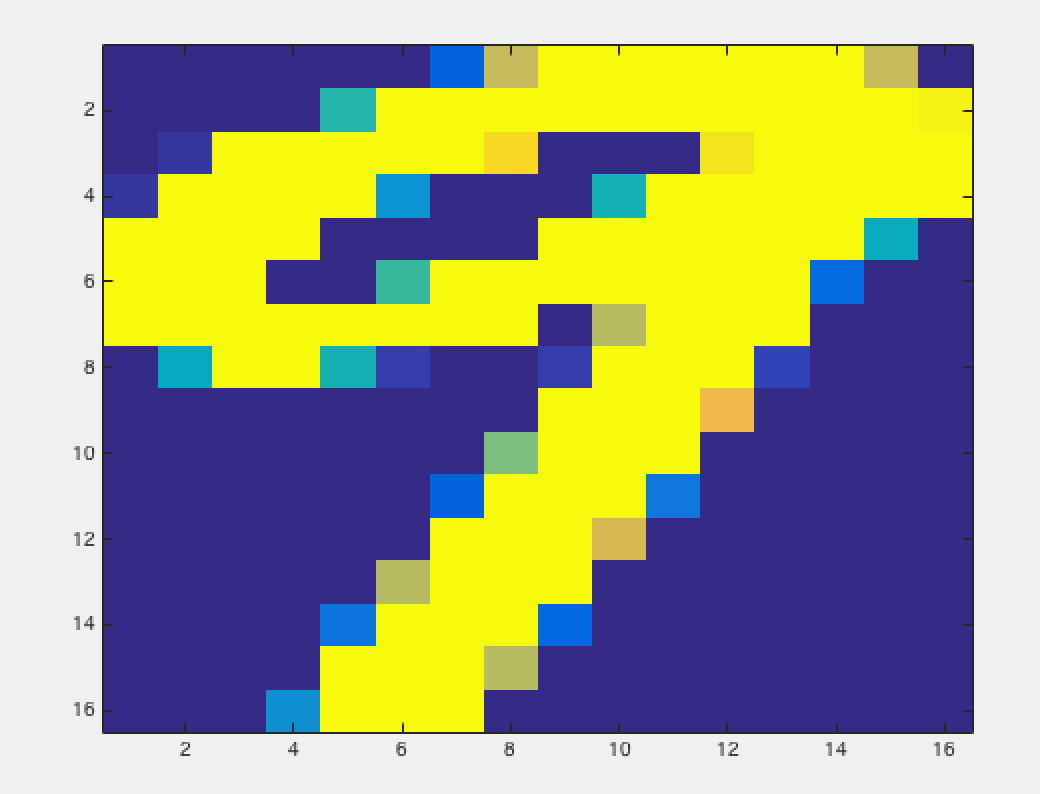
\includegraphics[width=0.25\textwidth, height=0.25\textwidth]{pic9}
\caption{Sample plots for each individual digits from 0 to 9. }
 \end{figure}
 \item 
To make sum of $x$ to be zero, then 
 \begin{align} 
\sum_{i=0}^{256}x_i &= \sum_{i=0}^{256}f_i + 256\gamma\\
&=0
 \end{align}
 Then \begin{align}  \gamma = -\frac{ \sum_{i=0}^{256}f_i}{256} 
 \end{align} 
 That means we just need to get summation of all values of all $1100$ pictures for each digit, and then divided by $256$.  \\
 
 
 \item 
 Totally there are $1100\times10$ images. For each image we can get the average of those $256$ pixels, and then subtract this average from the data image. 
 \begin{lstlisting}
%% Subtract the mean from each image 
residual =double(data) - repmat(mean(data),256, 1,1)
 \end{lstlisting} 
 
 \item 
 For each image matrix, we can get the singular values from Matlab SVD. The largest singular value is $  58194.51$. This is the global maximum singular value. \\ 
 \begin{lstlisting}
%% Reshape the matrix
m1 = reshape(residual, [256,11000])
[u,s, v] = svd(m1) 

 \end{lstlisting} 
 
\item 
The leading singular vector $\vu_1$ is shown as in Figure 2. \\
\begin{figure}
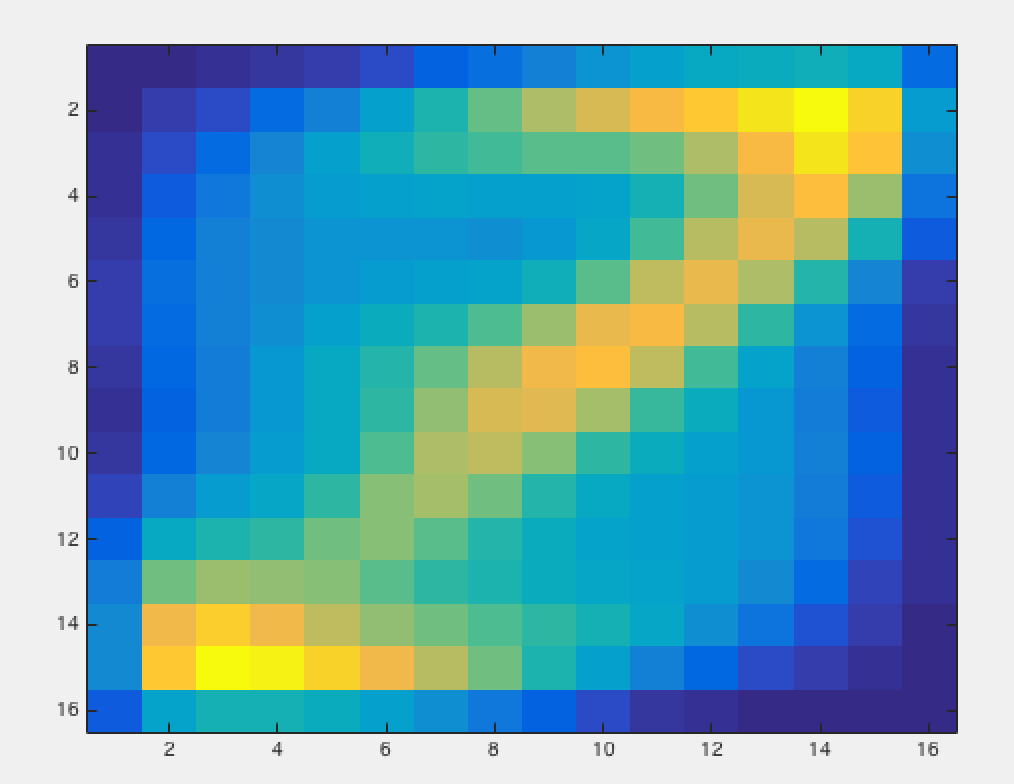
\includegraphics[width=0.5\textwidth]{prob4_4}
\centering
\caption{Plot of the leading singular vector $\vu_1$ for problem4.4 }

\end{figure}
\item 
The dominant eigenvalues for 10 matrices are: \\
$36414.5244628648	\\24385.2163297518	\\27837.9507648218	\\23367.3792733199	
\\25695.6406646778	\\ 27847.3481015609	\\26588.9227446172	\\26005.8518124203	\\26587.9255579203	\\33791.0691296690\\$

All the leading singular vectors are shown as in Figure 3. 
 \begin{figure}
 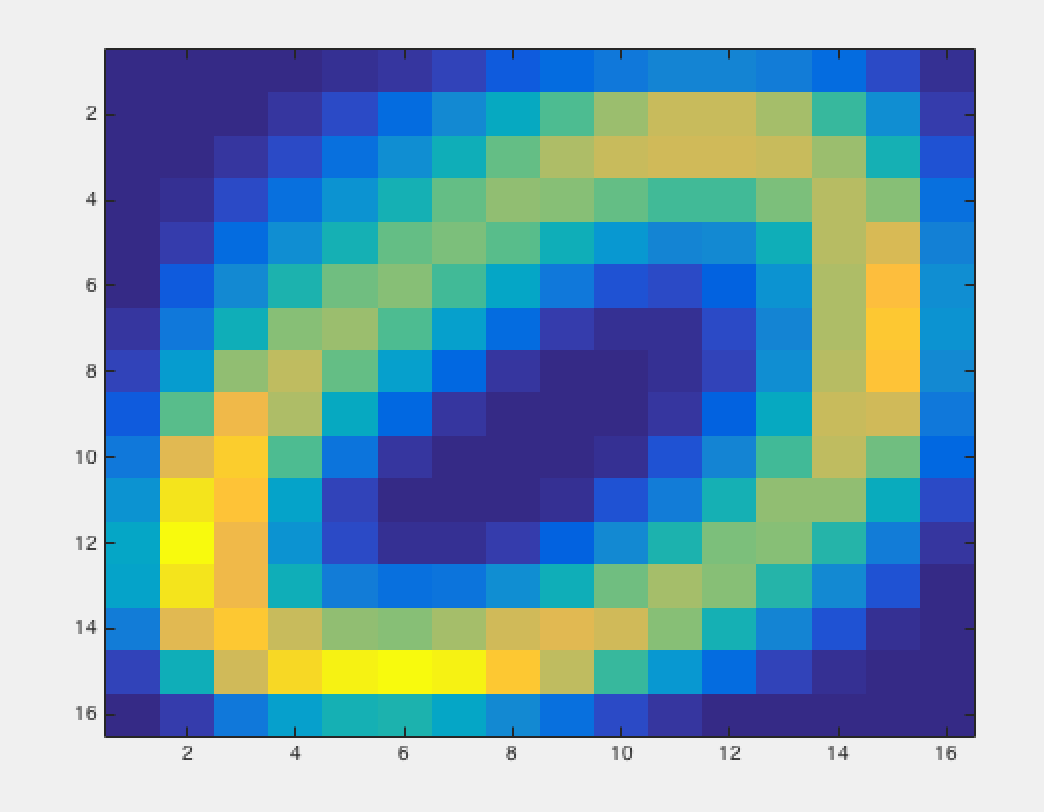
\includegraphics[width=0.25\textwidth, height=0.25\textwidth]{newpic0}
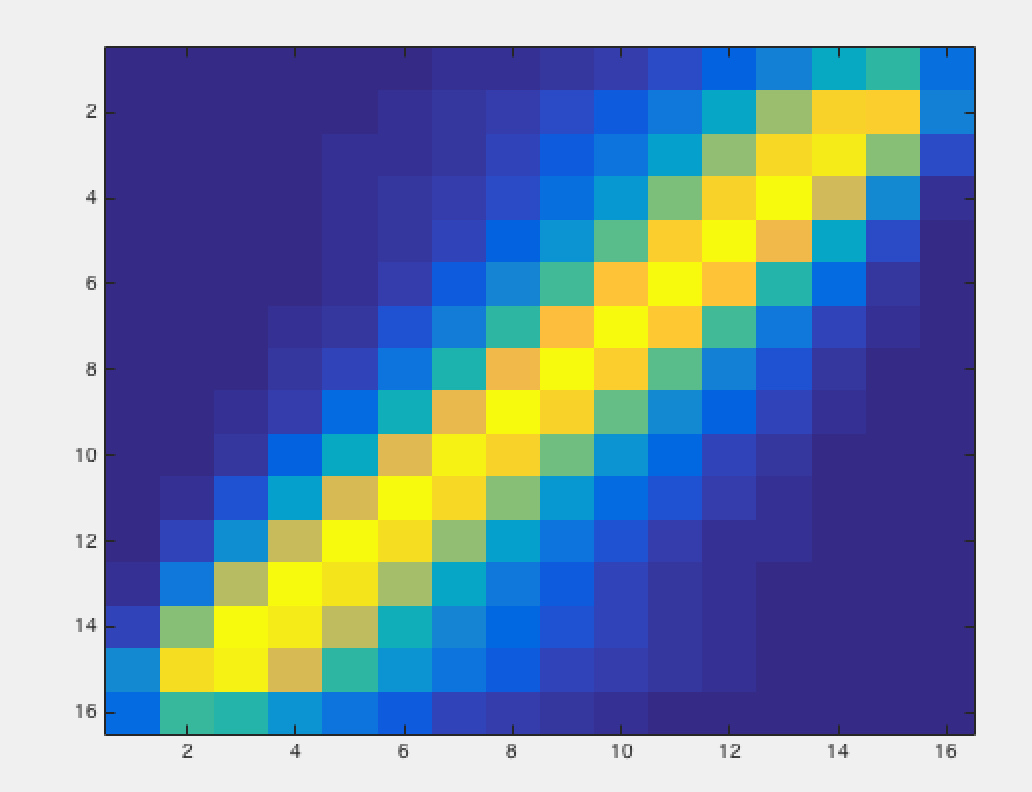
\includegraphics[width=0.25\textwidth, height=0.25\textwidth]{newpic1}   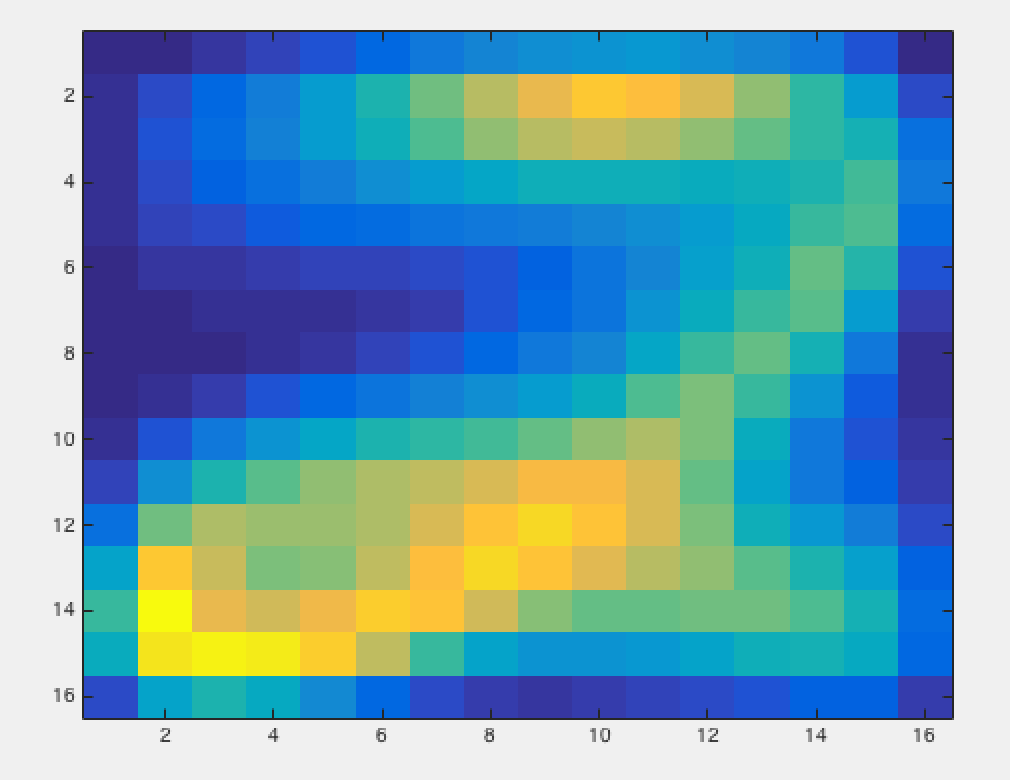
\includegraphics[width=0.25\textwidth, height=0.25\textwidth]{newpic2}
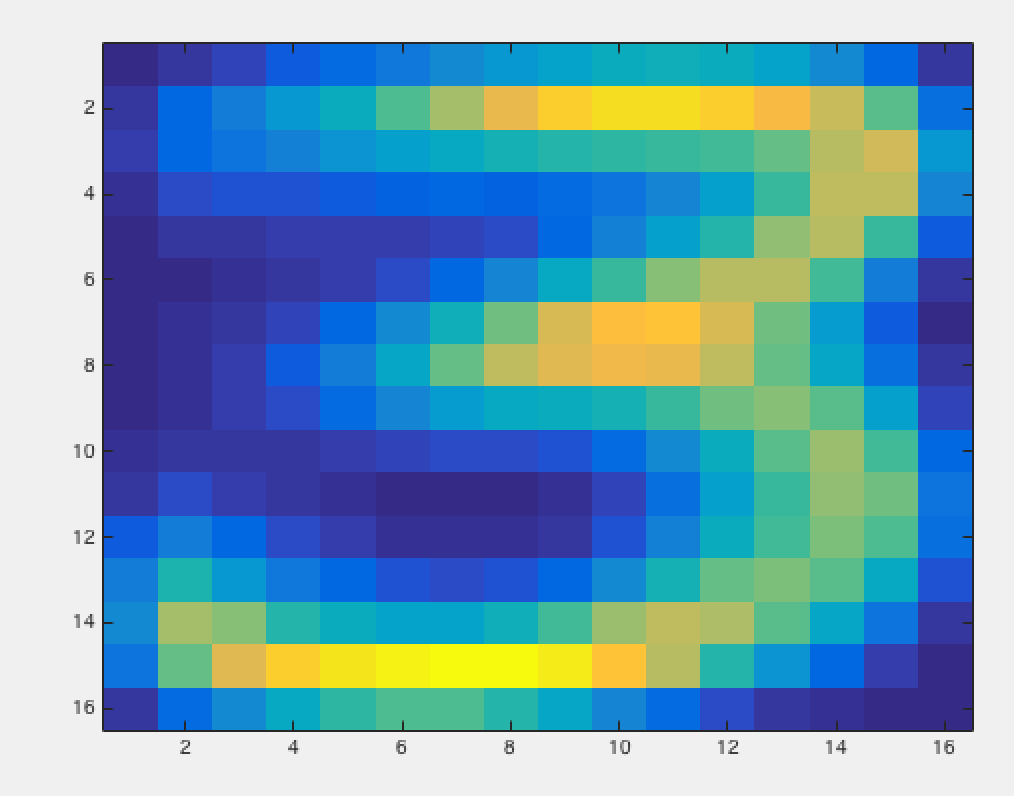
\includegraphics[width=0.25\textwidth, height=0.25\textwidth]{newpic3}
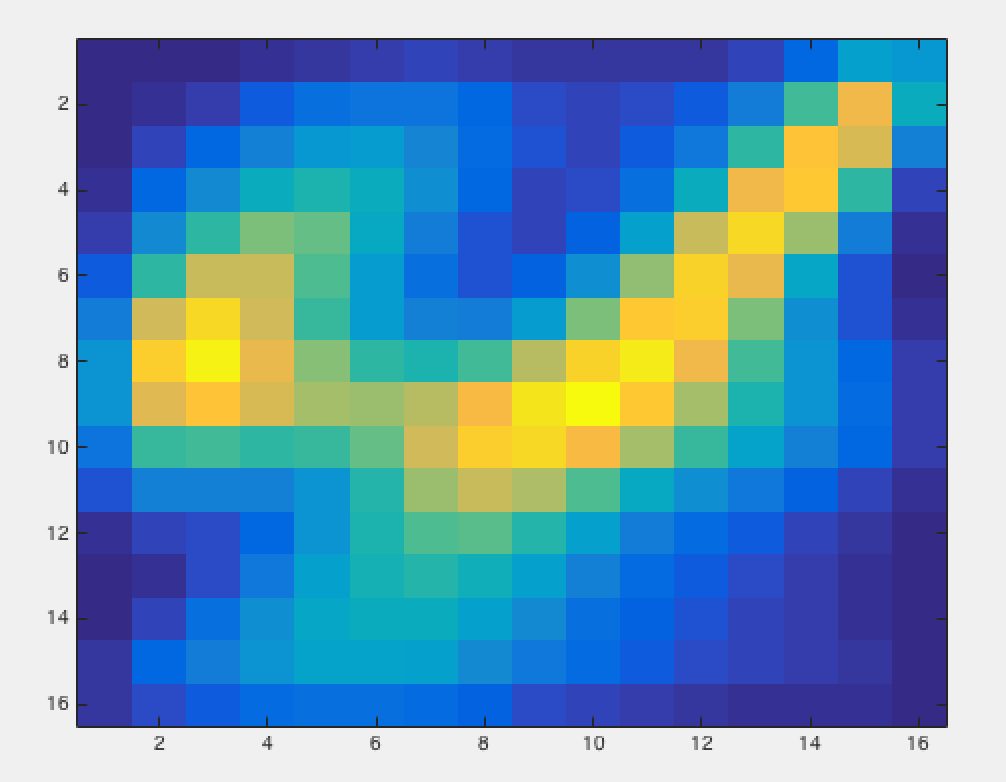
\includegraphics[width=0.25\textwidth, height=0.25\textwidth]{newpic4}
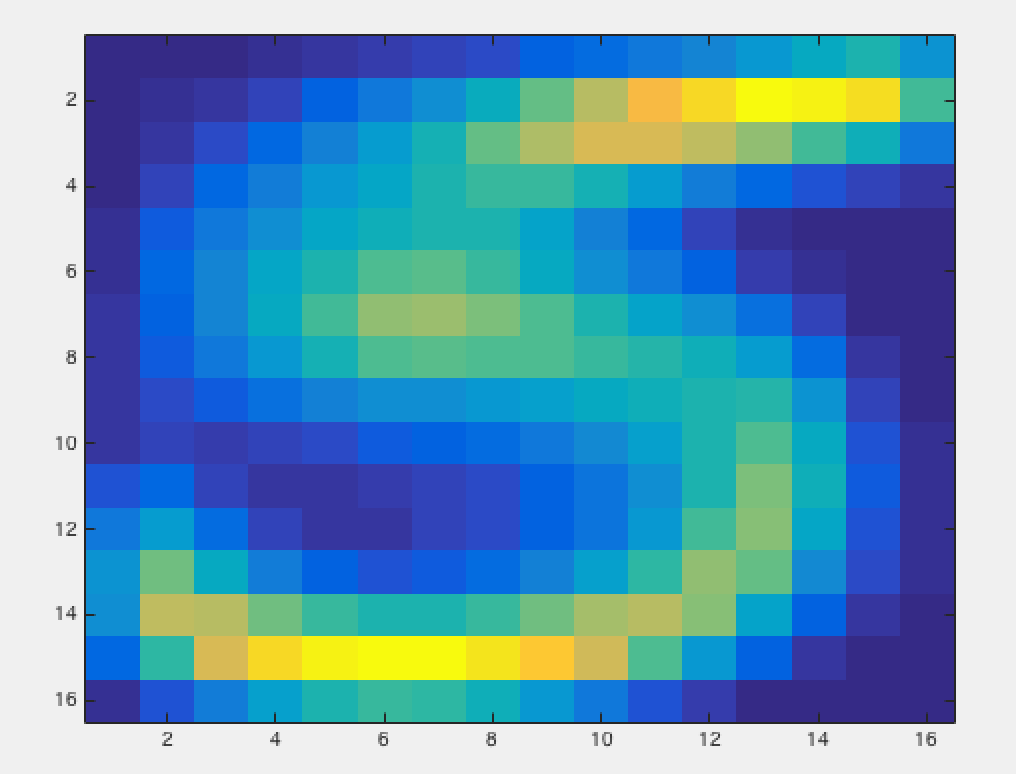
\includegraphics[width=0.25\textwidth, height=0.25\textwidth]{newpic5}
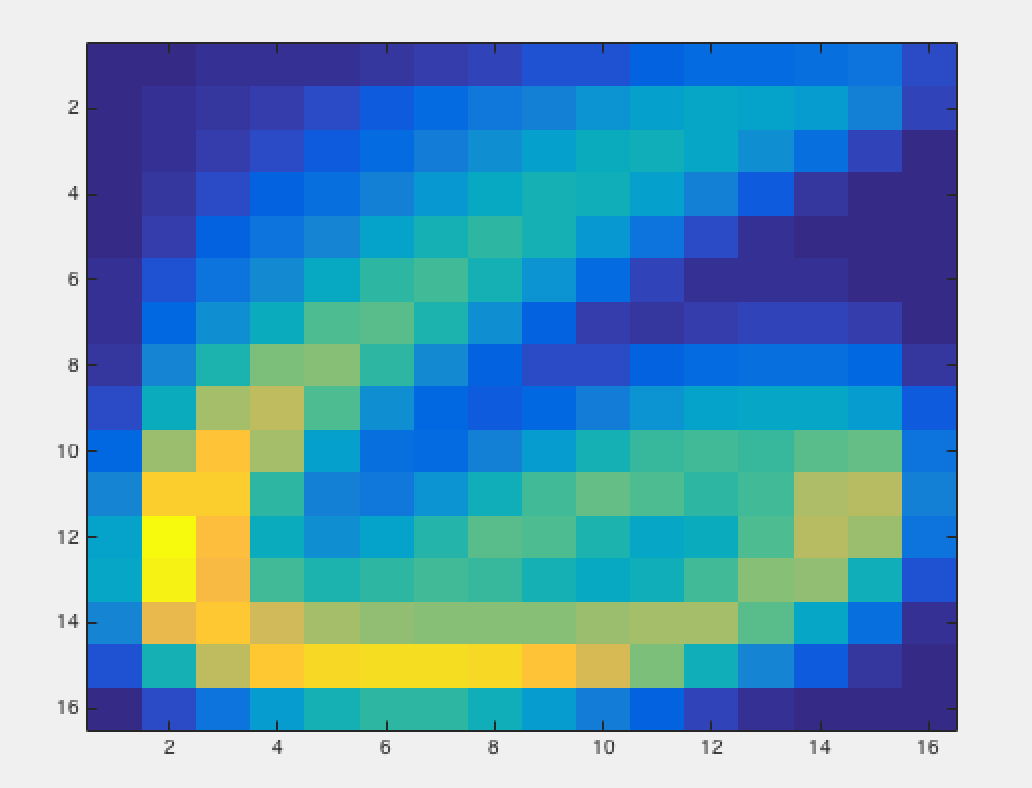
\includegraphics[width=0.25\textwidth, height=0.25\textwidth]{newpic6}
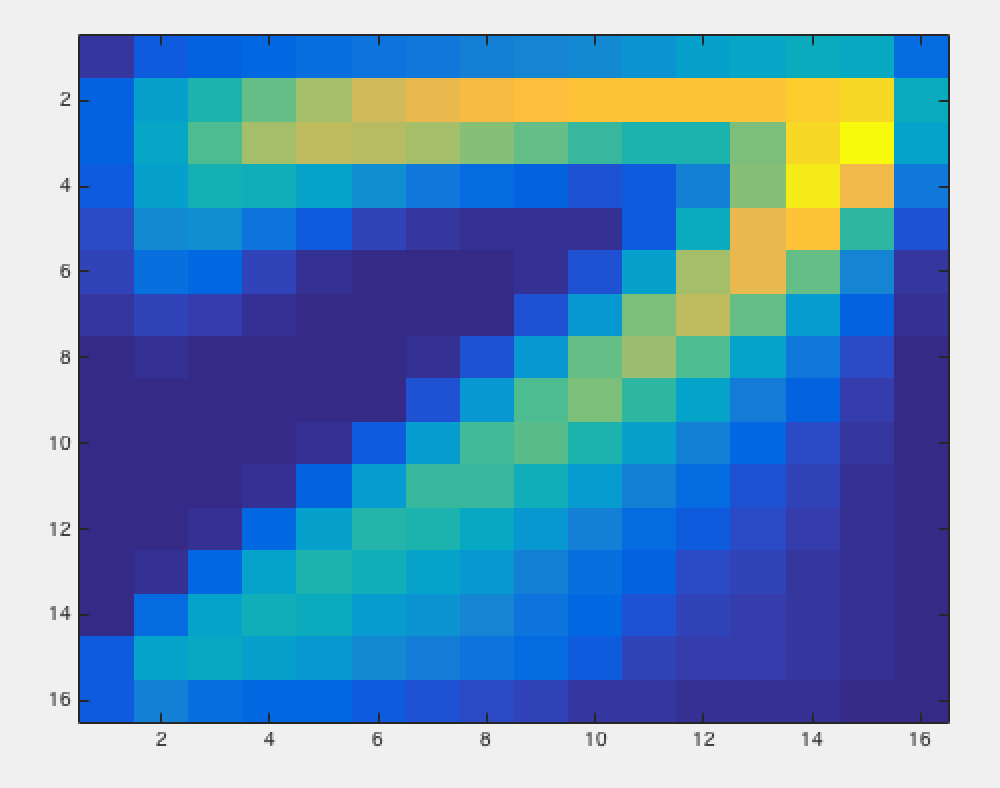
\includegraphics[width=0.25\textwidth, height=0.25\textwidth]{newpic7}
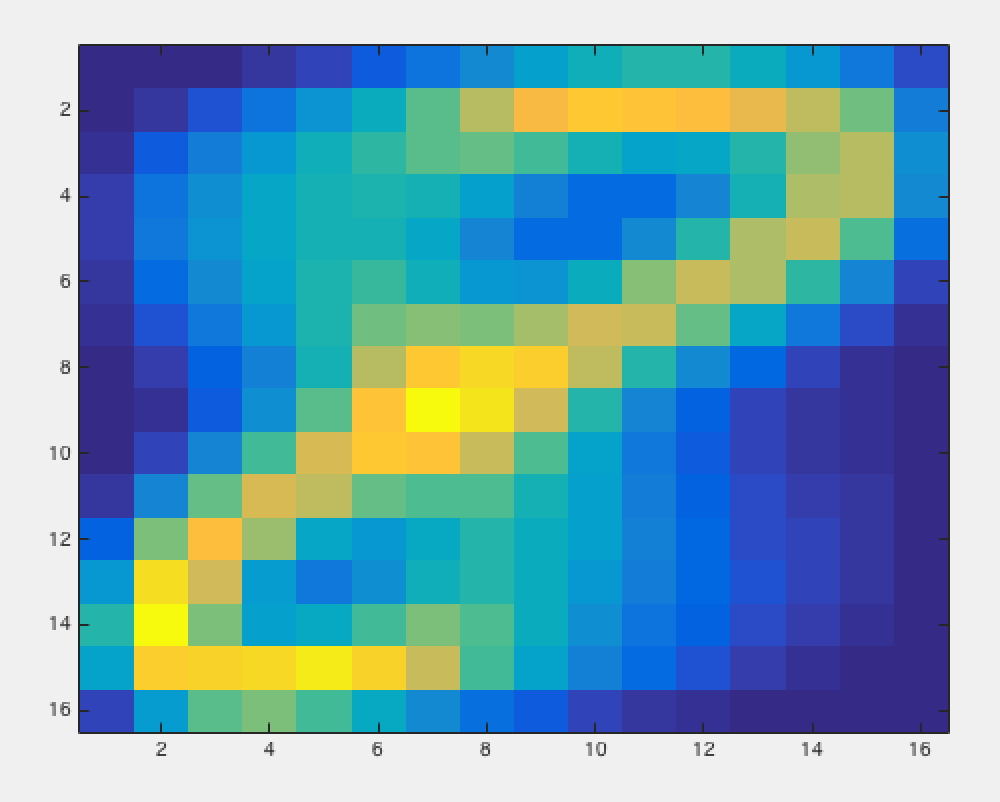
\includegraphics[width=0.25\textwidth, height=0.25\textwidth]{newpic8}
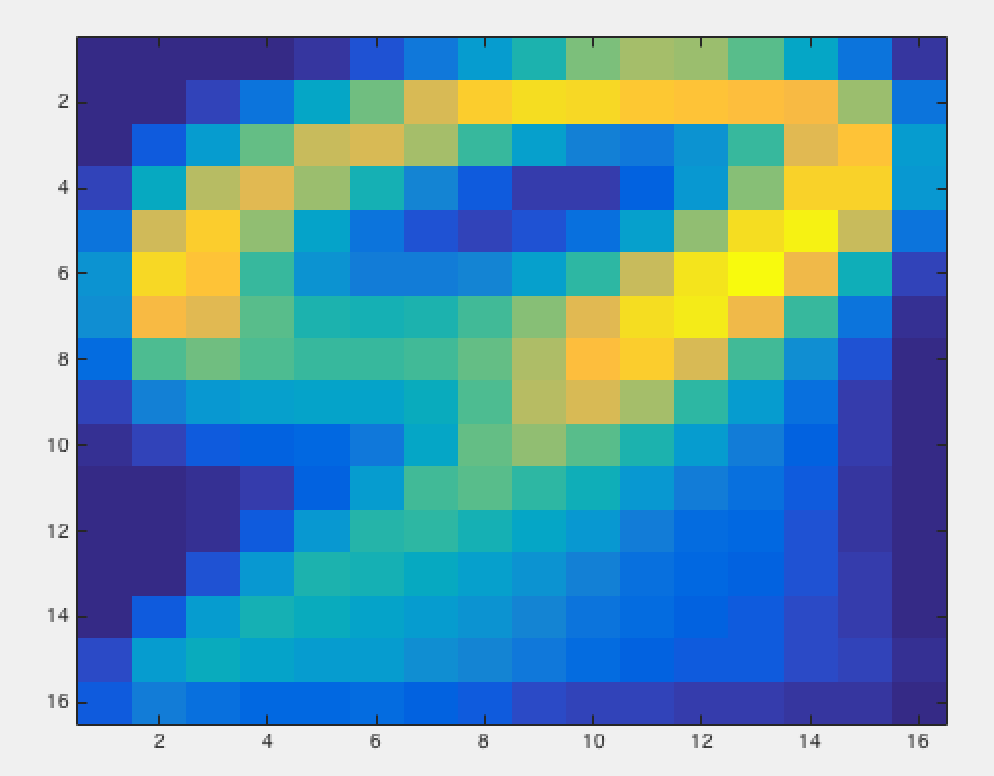
\includegraphics[width=0.25\textwidth, height=0.25\textwidth]{newpic9}
\caption{Plot of leading singular vectors for those 10 matrices }
 \end{figure}
 
 \begin{lstlisting}
mm = zeros(1,10); 
leadingV = zeros(256,10); 

for i=1:10
    [u,s,~] = svd(residual(:,:,i)); 
    mm(i)=s(1,1); 
    leadingV(:,i)=u(:,1); 
end
%% For example, plot the leading singular vector for digit 2. 
imagesc(reshape(leadingV(:, 2), [16,16]))
 \end{lstlisting}

The key difference is that the picture in number 5 include all features of digit 0 to 9.  But in this problem we can see that all the images contain its own digit features. 
\end{enumerate} 
\end{document}

